% !TeX root = text.tex
\documentclass{template/socthesis}

\usepackage{subcaption}
\usepackage{amsmath}
\usepackage{enumitem}

% my own code
\usepackage[skip=10pt plus1pt, indent=0pt]{parskip}

%%%%%% podbarvení bloků kódu / vygenerovaných ai
\usepackage{xcolor}
\usepackage{listings}
\usepackage{tcolorbox}
\tcbuselibrary{breakable}

\definecolor{aiblue}{rgb}{127,127,255}
\definecolor{aibackground}{rgb}{100,100,100}

\lstdefinestyle{aistyle}{
    backgroundcolor=\color{aibackground},   
    commentstyle=\color{aiblue},
    keywordstyle=\color{aiblue},
    numberstyle=\tiny\color{aiblue},
    stringstyle=\color{aiblue},
    basicstyle=\ttfamily\footnotesize,
    breakatwhitespace=false,         
    breaklines=true,                 
    captionpos=b,                    
    keepspaces=true,                 
    numbers=left,                    
    numbersep=5pt,                  
    showspaces=false,                
    showstringspaces=false,
    showtabs=false,                  
    tabsize=2
}

% https://tex.stackexchange.com/questions/24528/having-problems-with-listings-and-utf-8-can-it-be-fixed
\lstset{style=aistyle,
inputencoding=utf8,
extendedchars=true,
literate=%
{á}{{\'a}}1
{č}{{\v{c}}}1
{ď}{{\v{d}}}1
{é}{{\'e}}1
{ě}{{\v{e}}}1
{í}{{\'{\i}}}1
{ň}{{\v{n}}}1
{ó}{{\'o}}1
{ř}{{\v{r}}}1
{š}{{\v{s}}}1
{ť}{{\v{t}}}1
{ú}{{\'u}}1
{ů}{{\r{u}}}1
{ý}{{\'y}}1
{ž}{{\v{z}}}1
{Á}{{\'A}}1
{Č}{{\v{C}}}1
{Ď}{{\v{D}}}1
{É}{{\'E}}1
{Ě}{{\v{E}}}1
{Í}{{\'I}}1
{Ň}{{\v{N}}}1
{Ó}{{\'O}}1
{Ř}{{\v{R}}}1
{Š}{{\v{S}}}1
{Ť}{{\v{T}}}1
{Ú}{{\'U}}1
{Ů}{{\r{U}}}1
{Ý}{{\'Y}}1
{Ž}{{\v{Z}}}1
}

\addbibresource{text.bib}

\titlecz{Laserový projektor}
\titleen{Laser projector}
\author{Šimon Hrouda}
\field{10}
\school{Gymnázium Brno-Řečkovice}
\exmentor{Tomáš Rohlínek}
\exmentorstatement{Tomáše Rohlínka}
\inmentor{Mgr. Kateřina Vídenková}
\inmentorstatement{Mgr. Kateřiny Vídenkové}

% Změňte, pokud se liší
%\region{Jihomoravský}
\placefooter{Brno 2024}

\begin{document}
% \newcommand{\bard-gen}[3]{text vygenerován ai #1}
\newcommand{\bardgen}[3]{following text generated by ai (google bard) on #1\\%
  \begin{tcolorbox}[breakable, colback=blue!20]
    #2
  \end{tcolorbox}
  \begin{tcolorbox}[breakable, colback=blue!10, colframe=white]
    #3
  \end{tcolorbox}
}


\maketitle

\makecopyrightstatement{V~Brně}

\makethanks{Děkuji svému externímu konzultantovi Tomáši Rohlínkovi a své interní konzultantce Mgr. Kateřině Vídenkové za obětavou pomoc, podnětné připomínky a nekonečnou trpělivost, kterou mi během práce poskytovali.}

\pagestyle{empty}

\section*{Anotace}


\subsection*{Klíčová slova}


\vspace{20mm}

\section*{Annotation}


\subsection*{Keywords}


\newpage
\pagestyle{plain}

\tableofcontents % vysází obsah

%%% Začátek práce
\setcounter{figure}{0}
\setcounter{table}{0}
\newpage

\chapter*{Úvod}
\addcontentsline{toc}{chapter}{Úvod} % přidá položku úvod do obsahu
V této práci se zaměřuji na návrh a výrobu laserového projektoru, který za bude za pomoci páru zrcátek připevněných na galvanometrech rsychle měnit směr laserového paprsku a tím vykreslovat obraz na promítací plochu.


\newpage

definice pojmů a zkratek
\begin{center}
  \begin{tabular}{c c c}
    CLGS & Closed Loop Galvanometer System & systém galvanometru se zpětnou vazbou \\
    SPI & Serial Peripheral Interface & sériové periferní rozhraní \\
  \end{tabular}
\end{center}

\chapter{hardware}

\section{Raspberry Pi}

\section{Galvanometr a zrcátko}
\begin{itemize}
  \item
        Galvanometry, často nazývané galva, s časem nachází uplatnění ve více a více odvětvích práce s lasery.
        Oproti jiným možnostem nabízí flexibilitu, rychlost a přesnost za nízkou cenu.

        V práci používám galvanometry s uzavřenou smyčkou zpětné vazby (CLGS). (nikde nemůžu najít nejaky normalni rozdělení opne loop a closed loop, vsechny clanky mluvi rovnou o closed loop)
        V CLGS jsou potřeba 3 hlavní prvky, %pohybový akční člen, senzor a kontrolní desku - vycucáno z prstu

        Nejmodernější galvanometrové polohovací systémy jsou založené na principech elektromotorů s permanentními magnety, kde
        \cite{galva}
  \item
        \url{https://en.wikipedia.org/wiki/Galvanometer}\\
        \url{https://en.wikipedia.org/wiki/Laser_scanning}\\
        \url{https://en.wikipedia.org/wiki/Mirror_galvanometer}\\
        \url{https://en.wikipedia.org/wiki/Laser_lighting_display}

        A mirror galvanometer is an ammeter that indicates it has sensed an electric current by deflecting a light beam with a mirror.
        The mirror galvanometer consists of a long fine coil of silk-covered copper wire. %wtf silk == hedvábí??
        In the heart of that coil, within a little air-chamber, a small round mirror is hung by a single fibre of floss silk, with four tiny magnets cemented to its back
        The small weight of the mirror and magnets which form the moving part of this instrument, and the range to which the minute motions of the mirror can be magnified on the screen by the reflected beam of light, which acts as a long impalpable hand or pointer, render the mirror galvanometer marvellously sensitive to the current, especially when compared with other forms of receiving instruments.

        Zrcadlový galvanometr je měřič proudu, který reaguje na měřený proud vychýlením světelného paprsku zrcátkem připevněném na jeho konci.
        % Skládá se z dlouhé  tenké cívky měděného drátu potaženého hedvábím %wtf silk == hedvábí??
        % Ve středu této cívky je v malé vzduchové komůrce na jediném vláknu hedvábí

        Skládá se z cívky a
        \cite{zrcadlovy-galvanometr-wiki}

  \item
        \bardgen{2023-10-20}{popiš mi jak je sestaven a jak funguje galvanometr se zrcátkem k odrážení světelného paprsku}{
          Galvanometr se zrcátkem je sestaven z následujících komponent:

          * **Cívka:** Cívka je navinuta na jádře z feromagnetického materiálu, jako je železo nebo nikl. Cívkou prochází elektrický proud, který vytváří magnetické pole.
          * **Ukazatel:** Ukazatel je připojen k cívce a je vyroben z lehkého materiálu, jako je hliník nebo plast. Ukazatel je vychýlen magnetickým polem vytvářeným cívkou.
          * **Zrcátko:** Zrcátko je připojeno k ukazateli a odráží světelný paprsek.
          * **Okulár:** Okulár je umístěn tak, aby bylo možné pozorovat odraz světelného paprsku.

          **Jak funguje:**

          Když prochází cívkou elektrický proud, vytváří magnetické pole. Toto magnetické pole působí na ukazatel a vychýlí ho. Velikost výchylky ukazatele je přímo úměrná velikosti proudu procházejícího cívkou.

          Zrcátko je připojeno k ukazateli a odráží světelný paprsek. Když se ukazatel vychýlí, odraz světelného paprsku se také vychýlí.

          Okulár je umístěn tak, aby bylo možné pozorovat odraz světelného paprsku. Velikost vychýlení světelného paprsku je přímo úměrná velikosti proudu procházejícího cívkou.

          **Výhody:**

          * Galvanometr se zrcátkem je citlivější než galvanometr bez zrcátka.
          * Galvanometr se zrcátkem lze použít k měření velmi malých proudů.

          **Nevýhody:**

          * Galvanometr se zrcátkem je dražší než galvanometr bez zrcátka.

          **Použití:**

          Galvanometr se zrcátkem se používá k měření velmi malých proudů. Používá se například v elektrotechnice, lékařství a fyzice.
        }
\end{itemize}

ovládá se variabilním proudem

\section{hlavice}
\href{https://elenlaser.com/blog/galvo-head-laser-focus-tool.html}{The mirrors, mounted perpendicularly on the engines, move the laser beam along the X and Y axes according to the input received from the motor.
  The big advantage of these devices is that they can reach a very high acceleration and speed of movement.}
\section{řídící deska galv}
well asi patří do sekce galvanometr

\section{moje deska na napětí}
Galvanometry v obou osách pohybu potřebujeí analogový vstupní signál v rozpětí -15--+15~V udávající vychýlení galvanometru v daném směru.

Vytváření tohoto signálu jsem rozdělil do dvou částí, nejdříve pomocí DAC (digital-to-analog converter, D/A převodník) připojeného k RPi vytvořím signál v rozpětí 0--5~V a následně tento signál pomocí operačního zesilovače převedu na požadované rozpětí.
Celé zapojení je vidět na obrázku \ref{fig:dac_board}
\begin{figure}[!htb]
  \centering
  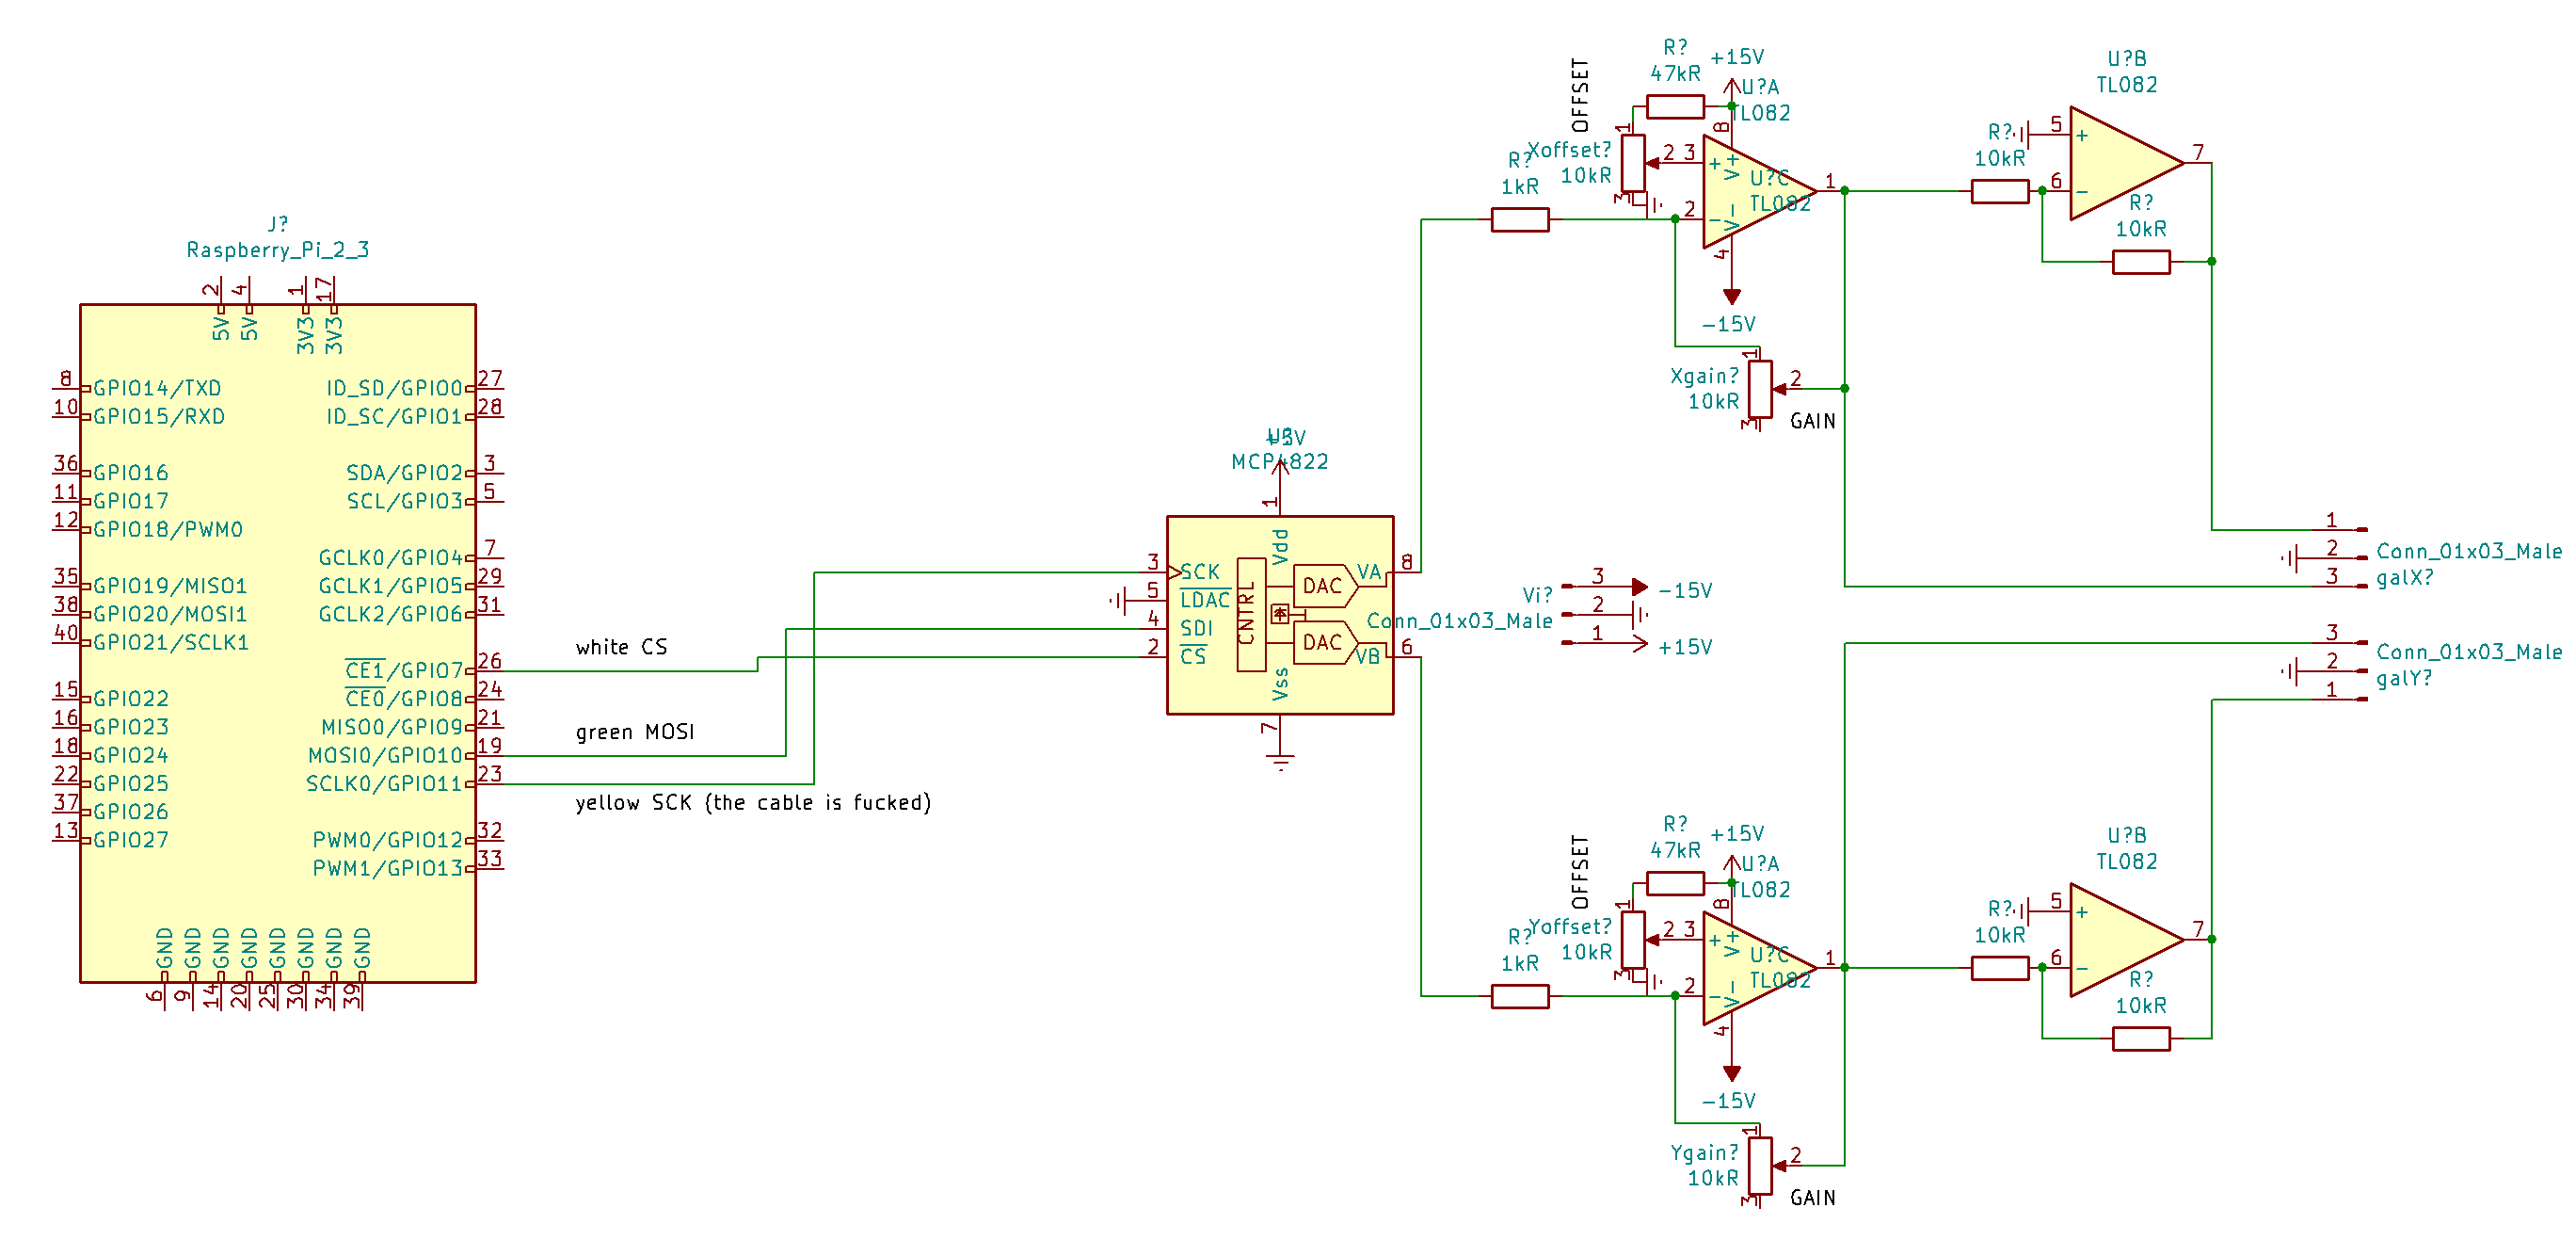
\includegraphics[width=1\textwidth]{img/dac_board.png} %unreadable text, make schem more compact
  \caption{\label{fig:dac_board}Zapojení DAC a zesilovačů k RPi a řídící desce galvanometrů}
\end{figure}

\subsection{dac}
K generování signálu v rozpětí 0--5V jsem využil DAC MCP4822 od firmy \href{https://www.microchip.com}{Microchip Technology Inc.}%TODO tečka?
Tento čip podporuje komunikaci přes rozhraní SPI, pracuje s napájecím napětím 5~V a s 12bitovým rozlišením (je schopen vygenerovat 4096 různých napětí) na dvou kanálech.

Komunikace mezi RPi a čipem je zprostředkována rozhraním SPI, toto rozhraní využívám pomocí knihovny ze serveru \url{https://github.com/pawel-kusinski/mcp4822-linux}; staženo 28.~12.~2023. %TODO tečka?
%TODO more spec
Tato knihovna poskytuje funkce \lstinline[language=C]!bool mcp4822_initialize();bool mcp4822_set_voltage(mcp4822_channel_t channel, uint16_t value_mV);void mcp4822_deinitialize();!, se kterými pracuji v mém kódu.
\subsection{amps}
K rozšíření signálu z DAC jsem využil dva operační zesilovače TL082 od firmy \href{https://www.ti.com/}{Texas Instruments Incorporated}. Každý z nich je připojený na jeden kanál DAC čipu mcp4822.
%TODO more spec
Tyto čipy mi napěťové rozpětí zvýší z 0--5~V na -15--+15~V.

\section{laser}
\section{if rgb: 3 dacs}


%TODO cos udelal svyho vlastne a jak to facha

\section{napájení}
%TODO ay tak co, zvladls to dat na baterky?

\chapter{software}
\section{lasershow exec}
\section{lcd + encoder}
\section{web ui}
\section{discord bot}
\section{HOTSPOT}

%TODO udelals to vubec dobre? porovnej se s ostatnima
\chapter{Diskuze}
\section{další zpracování tématu}
udelal jsem to dobre? vybral jsem si dobry technky?
like byl by lepsi ten harddrive z yt?
nebo fakt to melo byt napajeny z baterek a ne ze zasuvky?

ze hej ze \href{https://dspace.vutbr.cz/bitstream/handle/11012/38621/final-thesis.pdf?sequence=-1}{typek z vut} udelal kinda kurva podobnej HW jak ja, ale ja to mam trochu jinak, cuz jsem o tom nevedel, ale ofc moje je lepsi :))
also to delala hromada dalsich lidi na internetu ten hw, also od gh.com/tteskac mam executable, kterou jsem ale totalne ze rozsiril a taky jsem pridal vsechno moje genialni ui muhahahah

\B{ze este dalsi zpracovani: (19.10.2023 vsechny dostupne)}
\begin{enumerate}
  \item used/modified code
        \begin{itemize}
          \item \url{https://github.com/marcan/openlase/blob/master/tools/svg2ild.py}
          \item \url{https://github.com/tteskac/rpi-lasershow}
          \item \url{https://github.com/sabhiram/raspberry-wifi-conf/blob/master/app/wifi_manager.js}
          \item \url{http://www.electronicayciencia.com/wPi_soft_lcd/}
          \item \href{https://dspace.vutbr.cz/bitstream/handle/11012/38621/final-thesis.pdf?sequence=-1}{typek z vut}
        \end{itemize}
  \item dalsi zpracovani stejny projekty
        \begin{itemize}
          \item \url{https://www.instructables.com/Arduino-Laser-Show-With-Real-Galvos/}
          \item \url{https://github.com/tteskac/rpi-lasershow}
          \item \url{https://www.instructables.com/DIY-STEPDIR-LASER-GALVO-CONTROLLER/}
          \item \href{https://youtu.be/u9TpJ-_hBR8?si=mHy-UrptZZJ0Xu5-}{borec na yt hard-drive text gut}
        \end{itemize}
  \item other useful thingies
        \begin{itemize}
          \item \url{https://hackaday.io/project/172284-galvo-laser-cutterengraver}

          \item \url{https://hackaday.io/project/172284/instructions}

          \item \url{https://learn.adafruit.com/mcp4725-12-bit-dac-with-raspberry-pi/hooking-it-up}
          \item \url{https://www.ilda.com/resources/StandardsDocs/ILDA_IDTF14_rev011.pdf}
          \item cool demos \url{https://marcan.st/projects/openlase/}
          \item \url{https://www.youtube.com/watch?v=u9TpJ-_hBR8}
        \end{itemize}
  \item read
        \begin{itemize}
          \item \url{https://www.laserworld.com/en/glossary-definitions/90-t/2797-ttl-modulation-en.html}
        \end{itemize}

\end{enumerate}

\newpage
\chapter*{Závěr}
\addcontentsline{toc}{chapter}{Závěr} %FIXME proc vsichni maji zaver v obsahu jako section, kdyz pak vypada, ze je pod posledni kapitolou??
%TODO závěr
proc vsichni maji zaver v obsahu jako section, kdyz pak vypada, ze je pod posledni kapitolou

\newpage
\printbibliography[title=Literatura]
\addcontentsline{toc}{section}{Literatura}

\listoffigures
\addcontentsline{toc}{section}{Seznam obrázků}

\listoftables
\addcontentsline{toc}{section}{Seznam tabulek}
%
% \listoflistedequation
% \addcontentsline{toc}{section}{Seznam rovnic}

\end{document}
